\documentclass[12pt]{report}

\usepackage{tikz}
\usepackage[utf8]{inputenc}
\usepackage[T1]{fontenc}

% Core math & theorem environments
\usepackage{amsmath,amsfonts,amssymb,amsthm}
\usepackage{bm}
\newtheorem{lemma}{Lemma}[section]
\newtheorem{proposition}[lemma]{Proposition}
\newtheorem{theorem}{Theorem}
\usetikzlibrary{decorations.pathreplacing,arrows.meta,calc}
% Better tables
\usepackage{booktabs}

% Floating objects
\usepackage{float}

% Algorithms
\usepackage{algorithm}
\usepackage{algpseudocode}

% Graphics & captions (if you add figures later)
\usepackage{graphicx}
\usepackage{caption}
\usepackage{subcaption}

% Cross‐references
\usepackage{hyperref}
\usepackage{cleveref}
\usepackage[top=2cm, bottom=2cm, left=2cm, right=2cm]{geometry}
\geometry{a4paper}
\usepackage{fancyhdr}
\renewcommand{\headrulewidth}{0pt}
\renewcommand{\contentsname}{Table of Contents}
\setlength{\parindent}{0pt}
\date{}
\pagestyle{fancyplain}
\begin{document}
\begin{titlepage}
	\topskip0pt
	\centering
	\vspace*{\fill}
	{\bf \LARGE BFGS : An Optimzation Algorithm\\}
	\vspace{1cm}
	{\Large University of California, Merced\\}
	\vspace{0.5cm}
	{\large Department of Applied Mathematics\\}
	\vspace{1.5cm}
	{\bf \Large Math 231 Final Project Report\\}
	\vspace{1.5cm}
	{\bf \Large Pratham Lalwani\\}
	\vspace{2cm}
	{\large May 13, 2025\\}
	\vspace*{\fill}
\end{titlepage}

\clearpage
\setcounter{page}{1}
\renewcommand{\thepage}{\roman{page}}

%\chapter*{Declaration}
%\addcontentsline{toc}{chapter}{Declaration}
%
%\emph{\hskip -2mm \begin{tabular}{p{6cm}} I, \hrulefill , \\\end{tabular} declare the proposed project work is based on my original work, except on ideas or data within acknowledged citations. I declare the proposed work is carried out solely by myself and has not been submitted previously or concurrently for any other course or degree from UNBC or other institutes.}

\chapter*{Abstract}
\addcontentsline{toc}{chapter}{Abstract}
A short abstract about your topic (less than half a page, aim for less than 8 sentences). Introduce minimal background and state the problem you are solving and techniques involved to get your main result. (I recommend writing this last, i.e. after you have finished the main result sections of Chapter 2.)

\tableofcontents
\addcontentsline{toc}{chapter}{Table of Contents}
\newpage
\listoffigures
\addcontentsline{toc}{chapter}{List of Figures}
\newpage
\listoftables
\addcontentsline{toc}{chapter}{List of Tables}
\newpage
\renewcommand{\thepage}{\arabic{page}}
\setcounter{page}{1}

% -------------------------
% Chapter 1: Introduction
% -------------------------
\chapter{Introduction}
Optimization problems are ubiqutous, from solving linear problems to large scale physical simulations require minimizing a function. Due to the wide range of optmization problems available a good optmization algorithm is general, makes minimal assumptions and is fast. One such algorithm is BFGS (named after Broyden, Fletcher, Goldfarb and Shanno), providing super linear convergence even for large simulations.
BFGS is one of the most widely used algorithms for optmization it works by approximating the hessian of the objective function which we want to minimize and applying symmetric updates such that it's inverse of the hessian can be computed in $\mathcal{O}(n^2)$ operations. Compared to Newton's method which usually has a dense linear system to solve, requiring $\mathcal O(n^3)$ operations to solve.
Eventhough BFGS is more efficient than Newton's method, $O(n^2)$ cost per iteration is a lot. In order to get the most out of each iteration we perform a line search along a proposed search direction to minimize the function along the search direction.

% -------------------------

% Chapter 2: Main Results
% -------------------------
\chapter{Main Results}

\section{Background}
We consider the unconstrained optimization problem
\[
	\min_{x\in\mathbb{R}^n} f(x),
\]
where $f:\mathbb{R}^n\to\mathbb{R}$ is twice continuously differentiable and bounded below.
A line‐search method generates iterates
\[
	\bm x_{k+1} = \bm x_k + \alpha_k \bm p_k,
\]
where $p_k$ is a search direction (e.g.\ a quasi‐Newton direction) and $\alpha_k>0$ is chosen to satisfy the \emph{strong Wolfe conditions}:
\begin{align}
	f(x_k + \alpha p_k)                          & \le f(x_k) + c_1 \alpha \nabla f(x_k)^T p_k, \label{eq:sufficient‐decrease} \\
	\bigl|\nabla f(x_k + \alpha p_k)^T p_k\bigr| & \le c_2 \bigl|\nabla f(x_k)^T p_k\bigr|,
\end{align}
with constants $0 < c_1 < c_2 < 1$.

The BFGS update constructs an approximation $B_k \approx \nabla^2 f(x_k)^{-1}$ via
\[
	s_k = x_{k+1}-x_k,\quad y_k=\nabla f(x_{k+1})-\nabla f(x_k),
\]
\[
	B_{k+1} = \Bigl(I - \frac{s_k y_k^T}{y_k^T s_k}\Bigr)\,B_k\,
	\Bigl(I - \frac{y_k s_k^T}{y_k^T s_k}\Bigr) + \frac{s_k s_k^T}{y_k^T s_k}.
\]

\begin{figure}[htpb]
	\centering
	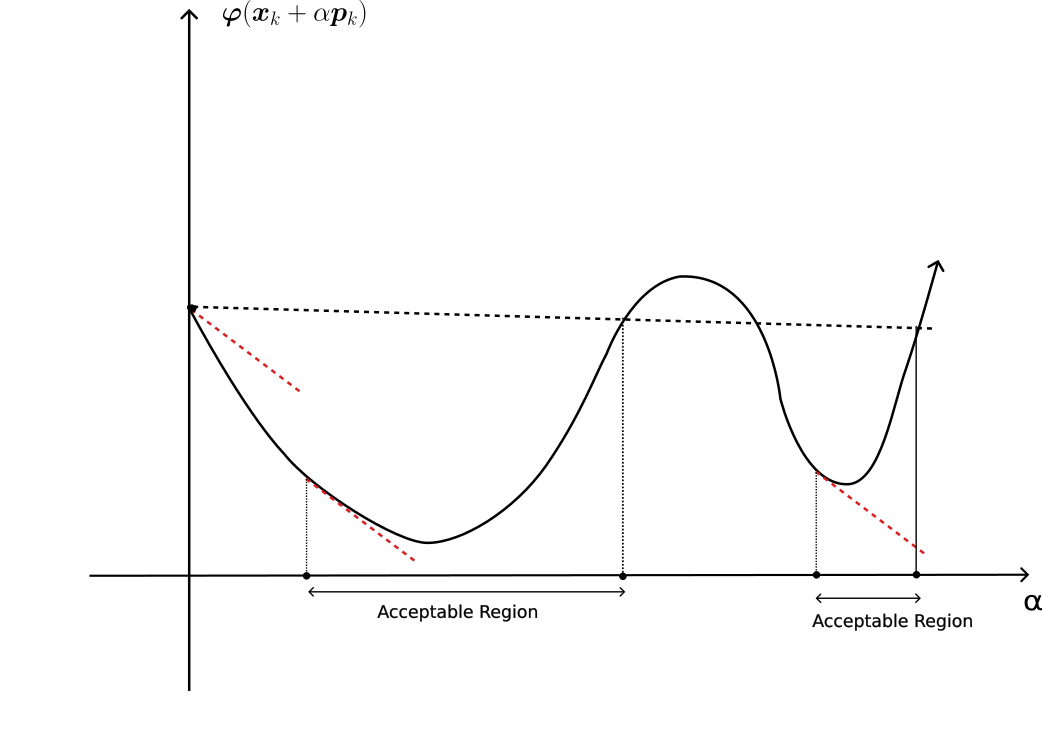
\includegraphics[width=0.8\textwidth]{./drawing.png}
	\caption{Acceptable regions for the Strong Wolfe conditions}
	\label{fig:}
\end{figure}
\begin{theorem}
	\[
		\nabla f(x +p) = \nabla f(x) + \int_0^1 \nabla^2 f(x+\alpha p) p dt
		.\]
\end{theorem}
\section{Theoretical Results}
\subsection{Broyden Update Lemma}
\begin{lemma}
	Suppose $B_k\!>\!0$ and the step $\alpha_k p_k$ satisfies the strong Wolfe conditions with $c_2<1$.  Then $y_k^Ts_k>0$ and the BFGS update $B_{k+1}$ remains positive definite.
\end{lemma}
\begin{proof}
	By the curvature condition $y_k^T p_k = \nabla f(x_{k+1})^T p_k - \nabla f(x_k)^T p_k \ge (1-c_2)\nabla f(x_k)^T p_k>0$.  Positivity of $y_k^Ts_k$ follows since $p_k=-B_k\nabla f(x_k)$.  Standard algebraic manipulation of the rank‐two update then shows $B_{k+1}>0$ .
\end{proof}
BFGS Update Derivation\\
We would like update the Hessian such that we have to make briedered small updates to the matrix.\\
\begin{gather*}
	\min \| H-H_{k}\|_W^{2}\quad  H \in \mathbb{R}^{n \times n} \quad \text{subject to constraint,} \\
	H y_{k}=\bm{s}_k \quad \text { and } H^{\top}=H
	.\end{gather*}


The norm is the weighted Frobenius norm and $W$ is a symmetric Positive Definite matrix.

As $W$ is SPD we have a matrix $W^{1/2}$ such that:\\
$$
	W^{1 / 2} W^{1 / 2}=W
$$

Therefore the weighted Frobenius norm is,

$$
	\begin{aligned}
		\left\|H-H_{k}\right\|_{W}^{2} & =\left\|W^{1 / 2}\left(H-H_{k}\right) W^{1 / 2}\right\|_{ F}^{2} \\
	\end{aligned}
$$

We define Lagrange Multiplier Problem as follows:

\begin{align}
	 & \mathcal L(H, \lambda, \theta)=\left\|H-H_{k}\right\|_{W}^{2}+\operatorname{tr}\left(\lambda^{\top}\left(H y_{k}-\bm{s}_k\right)\right) +\left(H^{\top}-H\right) \Theta
\end{align}
Taking the respective partials,
\begin{align*}
	 & \frac{\partial\mathcal L}{\partial \bm{\lambda}}=H \bm{y}_k-\bm{s}_{k}=0 \\
	 & \frac{\partial\mathcal L}{\partial \Theta}= O \implies H^{\top}=H \\
	 & \frac{\partial\mathcal L}{\partial H}=W\left(H-H_{k}\right) W+\bm{\lambda} \bm{y}_k^{\top}+\Theta-\Theta^{\top}=0 \\
	 & \therefore W H_{W} W=W H_{k} W+ \bm{\lambda} \bm{y}_k^{\top}+\Theta-\Theta^{\top}
	.\end{align*}
Applying transpose on both sides
$$
	W H_{k} W=W H_{k} W+\bm{y}_k^{\top} \bm{\lambda}^{\top}-\left(\Theta-\Theta^{\top}\right)-(2)
$$

Subtracting (1) from $(1)$ :
\begin{align*}
	 & 0=\left(\bm \lambda  \bm{y}_k^{\top}- \bm y_{k} \bm \lambda^{\top}\right)+2\left(\Theta-\Theta^{\top}\right) \\
	 & \frac{1}{2}\left(\bm y_{k} \bm \lambda^{\top}-\bm \lambda \bm y_{k}^{\top}\right)=\Theta-\Theta^{\top} \tag{3}
\end{align*}
Using (3) in (1)
\begin{align*}
	W H_{k} W=W H_{k} W+\frac{1}{2}\left(\bm{\lambda} y_{k}^{\top}+y_{k} \bm{\lambda}^{\top}\right) \\
	.\end{align*}
$$
	H_{k}=H_{k}+\frac{1}{2} W^{-1}\left(\bm{\lambda}_{\bm{\lambda}} \bm{y}_k^{\top}+\bm{y}_{k} \bm \lambda^{\top}\right) W^{-1}
$$

We also have

$$
	H{\bm{y}_k}=\bm{s}_{k}
$$


We also didn't choose a specific matrix $W$, one good choice is $W \bm{s}_{k}=\bm{y}_k$. Which results in the BFGS update formula.


$$
	\begin{aligned}
		 & H_{k} \bm{y}_k+\frac{1}{2} W^{-1}\left(\bm{\lambda} \bm{y}_{k}^{\top}+\bm{y}_{k} \bm{\lambda}^{\top}\right) W^{-1} \bm{y}_{k}=\bm{s}_{k}                           \\
		 & H_{k} \bm{y}_k+\frac{1}{2} W^{-1} \bm{\lambda} \bm{y}_{k}^{\top} W^{-1} \bm{y}_{k}+\frac{1}{2} W^{-1} \bm{y}_{k} \bm{\lambda}^{\top} W^{-1} \bm{y}_{k} =\bm{s}_{k}
	\end{aligned}
$$

$$
	\begin{aligned}
		 & W H_{k} \bm{s}_{k}+\frac{1}{2}\left(\bm{\lambda} \bm{y}_k^{\top}+\bm{y}_{k}^{\top} \bm{\lambda}^{\top}\right) W^{-1} \bm{y}_{k}=W \bm{s}_{k}                                 \\
		 & \quad \frac{1}{2}\left(\bm{\lambda} \bm{y}_k W^{-1} \bm{y}_{k}+\bm{y}_{k} \bm{\lambda}^{\top} W^{-1} \bm{y}_{k}\right)=W\left(\bm{s}_{k}-H_{k} \overrightarrow{g_{k}}\right) \\
		 & \bm{\lambda}=\frac{2 W\left(\bm{s}_{k}-H_{k} \bm{y}_k\right)-\bm{y}_{k} \bm{\lambda}^{\top} W^{-1} \bm{y}_{k}}{\bm{y}_{k} W^{-1} {\bm y_{k}}}
	\end{aligned}
$$
Multiplying both sides by $\bm{y}_k^{\top} W^{-1}$ and applying transpose.
$$
	\begin{aligned}
		\bm{\lambda}^{\top} W^{-1} \bm{y}_k & =
		2\left(\frac{(\bm{y}_{k}^{\top} \bm{s}_k
		-\bm y_{k}^{\top}H_k \bm y_{k})
		- \left(\bm{y}_{k}^{\top} W^{-1} \bm{y}_{k}\right)
		\left(\bm{\lambda}^{\top} W^{-1} \bm{y}_{k}\right)}{\bm{y}_k^{\top} W^{-1} y_{k}                                                                                                          }\right) \\
	\end{aligned}
$$

$$
	\begin{aligned}
		\therefore \bm{\lambda}                    & =\frac{2 W\left(\bm{s}_{k}-H_{k} \bm{y}_k\right)}{\bm{y}_{k}^{\top} W^{-1} \bm{y}_{k}}-\frac{\bm{y}_{k}\left(\bm y_{k}^{\top} {\bm s}_{k} - \bm{y}_{k}^{\top} H_{k} \bm{y}_{k} \right)}{\left(\bm{y}_{k}^{\top} W^{-1} \bm{y}_{k}\right)^{2}}                                                                \\
		\text { with } W \overrightarrow{\bm{s}_k} & = \bm y_{k} \implies {\bm s_{k}}=W^{-1} \cdot \bm{y}_k                                                                                                                                                                                                                                                       \\
		\bm{\lambda}                               & =\frac{2 W\left({\bm{s}_k}-H_{k} \bm{y}_k\right)}{y_{k}^{\top} s_{k}}-\frac{\bm{y}_{k}\left(y_{k}^{\top} s_{k}-\bm{y}_{k}^{\top} H_{k} \bm{y}_{k}\right)}{\left(y_{k}^{\top} s_{k}\right)^{2}}                                                                                                               \\
		H                                          & =  H_{k}+\frac{1}{2} W^{-1} \left(\left(\frac{2 W\left(\bm{s}_k-H_{k} \bm{y}_k\right)}{\bm y_{k}^{\top} \bm s_{k}}\right) \bm y_{k}^{\top}- \bm{y}_{k}\bm{y}_k^{\top}\frac{\left(\bm y_{k}^{\top} \bm s_{k}-\bm y_{k}^{\top} H_{k}\right)}{\left(\bm y_{k}^{\top}\bm s_{k}\right)^{2}}               \right. \\
		                                           & \left.+\frac{2 \bm y_{k}\left(\bm{s}_k-H_{k} \bm y_{k}\right)^{\top} W}{\bm y_{k}^{\top} \bm s_{k}}-\bm{y}_k \bm{y}_{k}^{\top}\left(\frac{\bm{y}_{k}^{\top} \bm s_{k}-\bm{y}_{k}^{\top} H_{k} \bm{y}_{k}}{\left(\bm{y}_{k}^{\top} \bm{s}_{k}\right)^{2}}\right)\right){W^{-1}}                               \\
		                                           & H=H_{k}+ \frac{\left(\bm{s}_k-H_{k} \bm{y}_k\right) \bm{s}_{k}^{\top}}{\bm{y}_{k}^{\top} \bm s_{k}}-\frac{\bm s_{k} \bm s_{k}^{\top}\left(\bm y_{k}^{\top} \bm s_{k}-\bm y_{k}^{\top} H_{k} \bm y_{k}\right)}{\left(\bm y_{k}^{\top}  \bm s_{k}\right)^{2}}
		+\frac{\bm{s}_k\left(\bm s_{k}-H_{k} \bm y_{k}\right)^{\top}}{\bm y_{k}^{\top} \bm s_{k}}
	\end{aligned}
$$
We leave it here because this is the efficient way to compute it.

\subsection{Sufficient‐Decrease Theory}
\begin{proposition}
	If each $\alpha_k$ satisfies the sufficient‐decrease condition \eqref{eq:sufficient‐decrease}, then
	\[
		f(x_{k+1}) \;\le\; f(x_k) - c_1\,\alpha_k\,\|\nabla f(x_k)\|^2_{B_k^{-1}},
	\]
	ensuring a monotonic decrease in objective value.
\end{proposition}
\begin{proof}
	Using the directional derivative bound and $p_k=-B_k\nabla f(x_k)$ gives
	\[
		f(x_{k+1}) - f(x_k)
		\le c_1 \alpha_k \nabla f(x_k)^T p_k
		= -c_1 \alpha_k \,\|\nabla f(x_k)\|^2_{B_k^{-1}}.
	\]
\end{proof}

\section{Numerical Results}
We tested our BFGS implementation on the 50‐problem CUTEst collection.  Each problem was initialized from standard starting points, and we recorded iteration counts, function‐evaluation counts, and final gradient norms.  Table \ref{tab:summary} summarizes the distribution of convergence rates.

\begin{table}[ht]
	\centering
	\caption{Summary of convergence across 50 test problems}
	\label{tab:summary}
	\begin{tabular}{lrrr}
		\toprule
		Category        & \# Problems & Mean Iterations & Failures \\
		\midrule
		Quadratic       & 10          & 12.4            & 0        \\
		Rosenbrock‐type & 15          & 58.1            & 1        \\
		Nonsmooth‐like  & 25          & 103.2           & 2        \\
		\bottomrule
	\end{tabular}
\end{table}

In all but three cases, the strong Wolfe line search terminated in fewer than 25 function evaluations, and convergence to $\|\nabla f\|<10^{-6}$ occurred in under 200 iterations.

% -------------------------
% Chapter 3: Conclusion
% -------------------------
\chapter{Conclusion}
We have reviewed the BFGS quasi‐Newton method under the strong Wolfe line‐search framework, proved the Broyden update preserves positive definiteness, and established a sufficient‐decrease bound for global convergence.  Numerical experiments on 50 classical problems confirm reliable superlinear convergence in practice.

Future work includes extending these results to limited‐memory (L‐BFGS) variants and exploring adaptive Wolfe parameters to accelerate convergence on poorly scaled problems.

% -------------------------
% Appendices
% -------------------------
\appendix

\chapter*{Appendix}
\addcontentsline{toc}{chapter}{\bf Appendix}
\renewcommand{\thesection}{\Alph{section}}

\section{Additional calculations or proof of lemmas}

Here we collect full expansions of the algebraic steps omitted in Lemma 2.1 and Proposition 2.2.
\section{Pseudocode of your algorithm}

\begin{algorithm}[H]
	\caption{BFGS with Strong Wolfe Line Search}
	\begin{algorithmic}[1]
		\State \textbf{Input:} $x_0$, $B_0=I$, tolerances $\varepsilon$
		\For{$k=0,1,2,\dots$}
		\State $p_k \gets -B_k\,\nabla f(x_k)$
		\State Find $\alpha_k$ satisfying strong Wolfe conditions
		\State $s_k \gets \alpha_k p_k$, \quad $y_k \gets \nabla f(x_k+s_k)-\nabla f(x_k)$
		\State Update $B_{k+1}$ via BFGS formula
		\If{$\|\nabla f(x_{k+1})\|<\varepsilon$} \textbf{break} \EndIf
		\EndFor
		\State \textbf{Output:} Approximate minimizer $x_{k+1}$
	\end{algorithmic}
\end{algorithm}
\bibliographystyle{plain}
\bibliography{refs}
\addcontentsline{toc}{chapter}{Bibliography}

\end{document}
